%%%%%%%%%%%%%%%%%%%%%%%%%%%%%%%%%%%%%%%%%
% Memo
% LaTeX Template
% Version 1.0 (30/12/13)
%
% This template has been downloaded from:
% http://www.LaTeXTemplates.com
%
% Original author:
% Rob Oakes (http://www.oak-tree.us) with modifications by:
% Vel (vel@latextemplates.com)
%
% License:
% CC BY-NC-SA 3.0 (http://creativecommons.org/licenses/by-nc-sa/3.0/)
%
%%%%%%%%%%%%%%%%%%%%%%%%%%%%%%%%%%%%%%%%%

\documentclass[letterpaper,11pt]{texMemo2} % Set the paper size (letterpaper, a4paper, etc) and font size (10pt, 11pt or 12pt)

\usepackage{parskip} % Adds spacing between paragraphs
\setlength{\parindent}{15pt} % Indent paragraphs
\usepackage[caption=false]{subfig}
%----------------------------------------------------------------------------------------
%	MEMO INFORMATION
%--------------------------------------------------------------------------------

%\memoto{Mr. Lynch } % Recipient(s)
%\memofrom{Mike Patel} % Sender(s)
%\memosubject{Staff Injury Report} % Memo subject
\space
\memodate{\today} % Date, set to \today for automatically printing todays date

%\logo{
\includegraphics[width=0.3\textwidth]{logo.png}} % Institution logo at the top right of the memo, comment out this line for no logo

%----------------------------------------------------------------------------------------

\begin{document}
	
	\maketitle % Print the memo header information
	
	%----------------------------------------------------------------------------------------
	%	MEMO CONTENT
	%----------------------------------------------------------------------------------------
	
	
	
	
	\section{Python Code}
	\begin{figure}[htp]
		\centering 
		
		%\subfloat[Create test.py]{%
			\includegraphics[clip,width=1\columnwidth,height=9cm]{1a}%
		
	\end{figure}
		\section{http://localhost:5000/test}
		\begin{figure}[htp]
		\centering 

		%\subfloat[Navigate to \textbf{localhost:5090}]]{%
			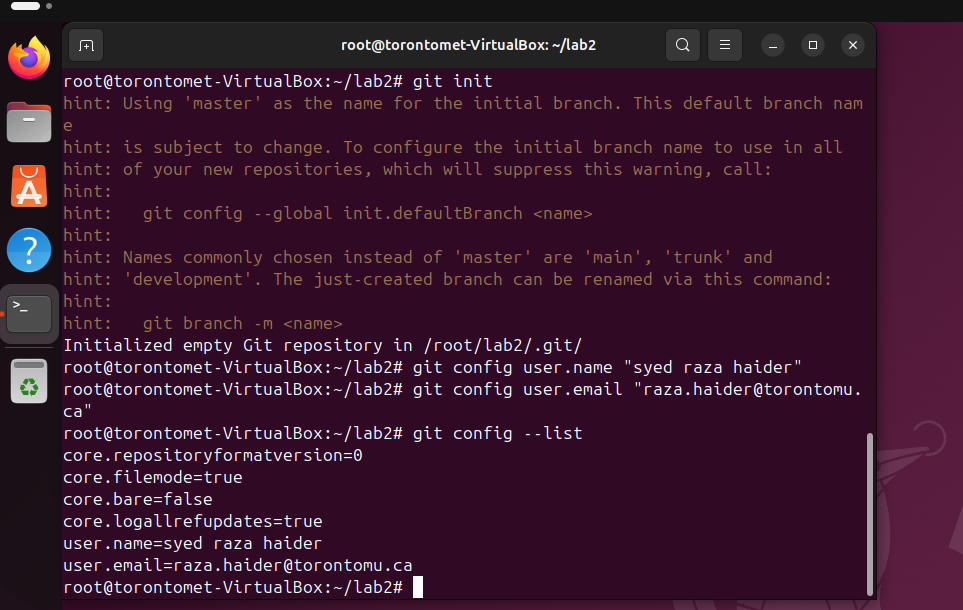
\includegraphics[clip,width=0.8\columnwidth,height=6cm]{2}%
			
			
		\end{figure}
	\newpage
	\section{MongoDB Compass and CKCS145 database with collection}
	\begin{figure}[htp]
		\centering 
		
		%\subfloat[Navigate to \textbf{localhost:5090/param}]]{%
			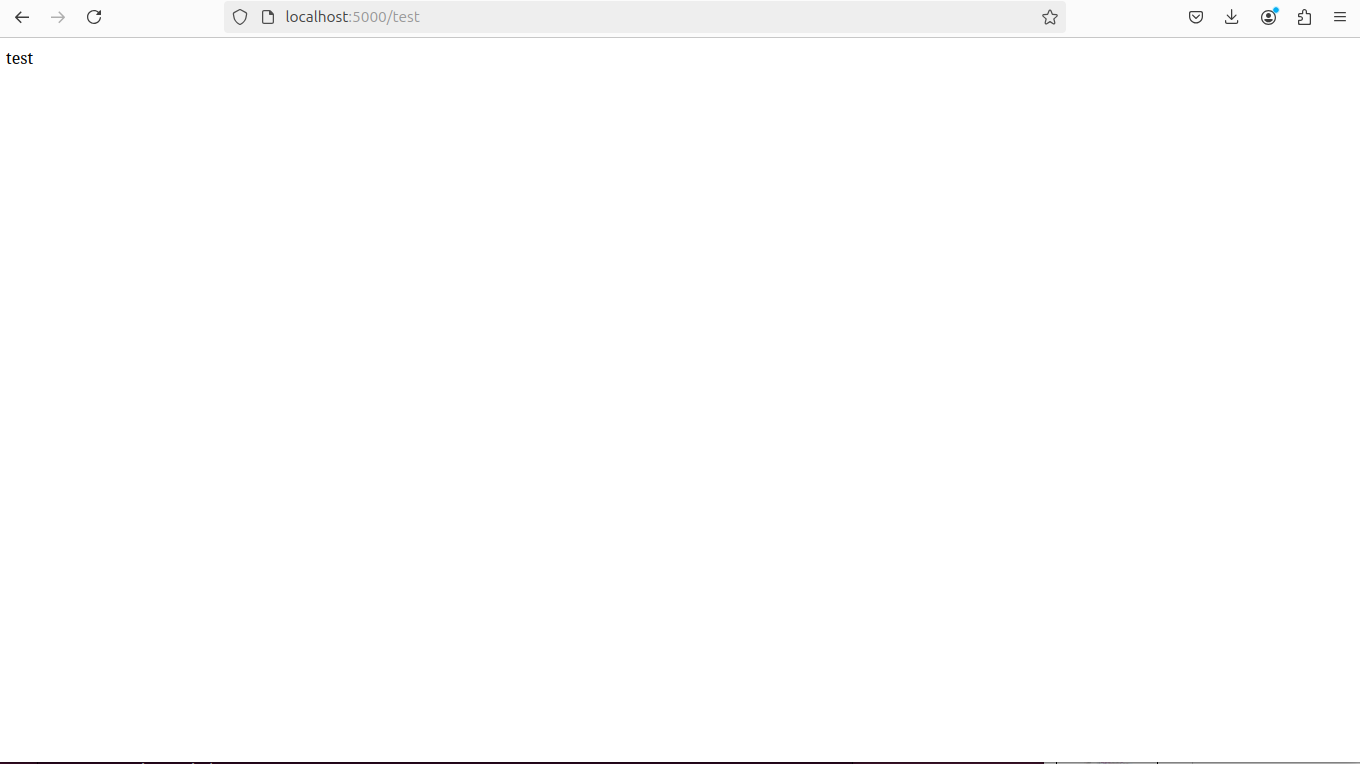
\includegraphics[clip,width=1.0\columnwidth,height=7cm]{3}%
		%}

	\end{figure}
	
		\section{http://localhost:5000/user/list}
	\begin{figure}[htp]
		\centering 
		
		%	\subfloat[Execute Code via terminal and open browser with path \textbf{localhost:5000}]{%
			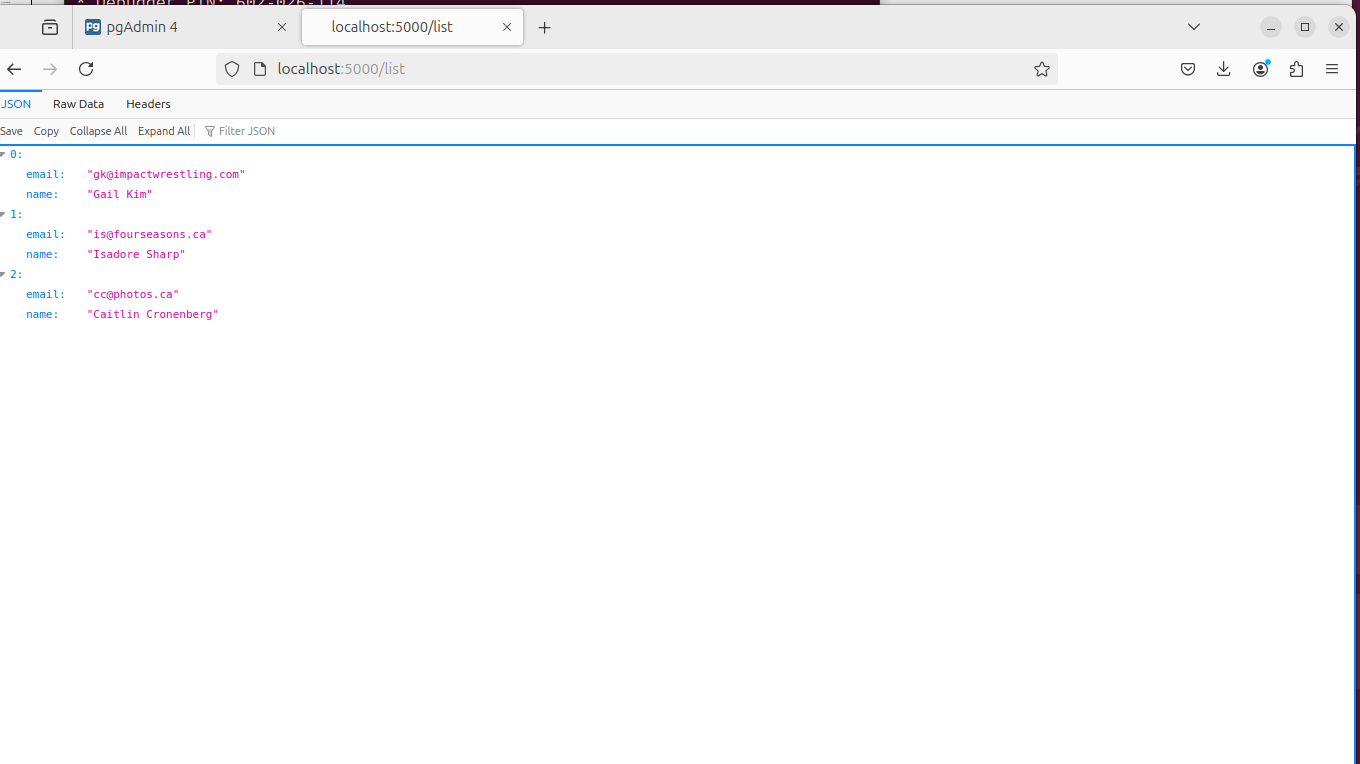
\includegraphics[clip,width=1.2\columnwidth,height=7cm]{4}%
			%	}
		
		
		
		%	\caption{Offshoring level. \\Source: Elaborated data from WIOT and SEA tables (2016).}
		
	\end{figure}
	\newpage
	\section{POST request using RESTer}
	
	\begin{figure}[htp]
		\centering 
		
		%\subfloat[Shows output function from python code \textbf{def test1()}]{%
			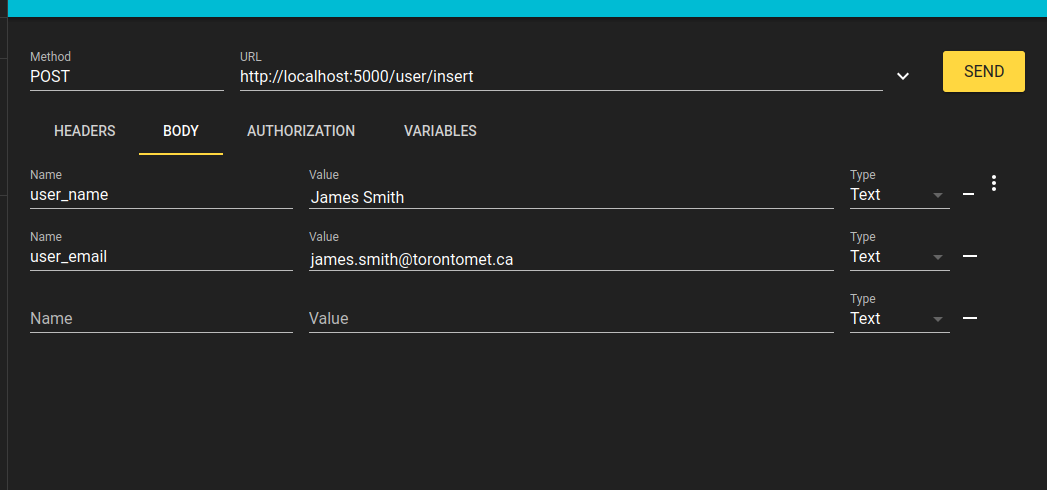
\includegraphics[clip,width=0.9\columnwidth,height=8cm]{5}%

		
	\end{figure}
	
		\section{MongoDB Compass and with updated CKCS145 database}
	
	\begin{figure}[htp]
		\centering 

		%	\subfloat[Create a text file named readme.txt]{%
			\includegraphics[clip,width=0.9\columnwidth,height=8cm]{6a}%
			%}
		
		%Navigate to \textbf{localhost:5000/param}
		
		%	\caption{Offshoring level. \\Source: Elaborated data from WIOT and SEA tables (2016).}
		
	\end{figure}
	%\newpage
	%----------------------------------------------------------------------------------------
	\section{In this lab, only GET and POST requests are used. Why are PUT and DELETE requests not used?}
	 The lab uses GET and POST for simplicity and compatibility, while PUT and DELETE are not needed for the basic scenarios covered in the lab.
	
\end{document}